%++++++++++++++++++++++++++++++++++++++++
\documentclass[article, 12pt]{article}
\usepackage{float}
\usepackage{setspace}
\usepackage{tabu} % extra features for tabular environment
\usepackage{amsmath}  % improve math presentation
\usepackage{graphicx} % takes care of graphic including machinery
\usepackage[margin=1in]{geometry} % decreases margins
\usepackage{cite} % takes care of citations
\usepackage[final]{hyperref} % adds hyper links inside the generated pdf file
\usepackage{tikz}
\usepackage{caption} 
\usepackage{fancyhdr}
\usepackage{amssymb} % symbols like /therefore
\usepackage{amsthm} % proofs
\usepackage{enumerate} % lettered lists
\usepackage{mathtools} % macros
\usepackage{multirow} % multirow tables
\usepackage{pgfplots} % plots
\usetikzlibrary{scopes}
% \usepackage{xcolor} \pagecolor[rgb]{0.12549019607,0.1294117647,0.13725490196} \color[rgb]{0.82352941176,0.76862745098,0.62745098039} % dark theme
\hypersetup{
	colorlinks=true,       % false: boxed links; true: colored links
	linkcolor=blue,        % color of internal links
	citecolor=blue,        % color of links to bibliography
	filecolor=magenta,     % color of file links
	urlcolor=blue         
}
\usepackage{physics}
\usepackage{siunitx}
\usepackage{tikz,pgfplots}
\usepackage[outline]{contour} % glow around text
\usetikzlibrary{calc}
\usetikzlibrary{angles,quotes} % for pic
\usetikzlibrary{arrows.meta}
\tikzset{>=latex} % for LaTeX arrow head
\contourlength{1.2pt}

\colorlet{xcol}{blue!70!black}
\definecolor{babyblueeyes}{rgb}{0.63, 0.79, 0.95}
\colorlet{vcol}{green!60!black}
\colorlet{myred}{red!70!black}
\colorlet{myblue}{blue!70!black}
\colorlet{mygreen}{green!70!black}
\colorlet{mydarkred}{myred!70!black}
\colorlet{mydarkblue}{myblue!60!black}
\colorlet{mydarkgreen}{mygreen!60!black}
\colorlet{acol}{red!50!blue!80!black!80}
\tikzstyle{CM}=[red!40!black,fill=red!80!black!80]
\tikzstyle{xline}=[xcol,thick,smooth]
\tikzstyle{mass}=[line width=0.6,red!30!black,fill=red!40!black!10,rounded corners=1,
                  top color=red!40!black!20,bottom color=red!40!black!10,shading angle=20]
\tikzstyle{faded mass}=[dashed,line width=0.1,red!30!black!40,fill=red!40!black!10,rounded corners=1,
                        top color=red!40!black!10,bottom color=red!40!black!10,shading angle=20]
\tikzstyle{rope}=[brown!70!black,very thick,line cap=round]
\def\rope#1{ \draw[black,line width=1.4] #1; \draw[rope,line width=1.1] #1; }
\tikzstyle{force}=[->,myred,very thick,line cap=round]
\tikzstyle{velocity}=[->,vcol,very thick,line cap=round]
\tikzstyle{Fproj}=[force,myred!40]
\tikzstyle{myarr}=[-{Latex[length=3,width=2]},thin]
\def\tick#1#2{\draw[thick] (#1)++(#2:0.12) --++ (#2-180:0.24)}
\DeclareMathOperator{\sn}{sn}
\DeclareMathOperator{\cn}{cn}
\DeclareMathOperator{\dn}{dn}
\def\N{80} % number of samples in plots


\usepackage{titling}
\renewcommand\maketitlehooka{\null\mbox{}\vfill}
\renewcommand\maketitlehookd{\vfill\null}
\usepackage{siunitx} % units
\usepackage{verbatim} 
\usepackage[outline]{contour} % glow around text

\newcommand{\labTitle}{Slinky and Magnetic Field Lab}
\newcommand{\class}{AP Physics C}
\newcommand{\professor}{Mr. Perkins}
\newcommand{\name}{Denny Cao}
\pagestyle{fancy}
\fancyhf{}% clears all header and footer fields
\fancyfoot[C]{--~\thepage~--}
\renewcommand*{\headrulewidth}{0.4pt}
\renewcommand*{\footrulewidth}{0pt}
\lhead{\name}
\chead{\class: \labTitle}
\rhead{\professor}


\fancypagestyle{plain}{%
  \fancyhf{}% clears all header and footer fields
  \fancyfoot[C]{--~\thepage~--}%
  \renewcommand*{\headrulewidth}{0pt}%
  \renewcommand*{\footrulewidth}{0pt}%
}

% Shortcuts
\DeclarePairedDelimiter\ceil{\lceil}{\rceil} % ceil function
\DeclarePairedDelimiter\floor{\lfloor}{\rfloor} % floor function

\DeclarePairedDelimiter\paren{(}{)} % parenthesis

\newcommand{\df}{\displaystyle\frac} % displaystyle fraction
\newcommand{\qeq}{\overset{?}{=}} % questionable equality

\newcommand{\Mod}[1]{\;\mathrm{mod}\; #1} % modulo operator

% Sets
\DeclarePairedDelimiter\set{\{}{\}}
\newcommand{\unite}{\cup}
\newcommand{\inter}{\cap}

\newcommand{\reals}{\mathbb{R}} % real numbers: textbook is Z^+ and 0
\newcommand{\ints}{\mathbb{Z}}
\newcommand{\nats}{\mathbb{N}}
\newcommand{\rats}{\mathbb{Q}}

\newcommand{\degree}{^\circ}
\newcommand{\tplint}[6]{\int\limits^{#1}_{#2}\int\limits^{#3}_{#4}\int\limits^{#5}_{#6}} % triple integral bounds
% Counting
\newcommand{\dblint}[4]{\int\limits^{#1}_{#2}\int\limits^{#3}_{#4}} % double integral bounds
\newcommand{\sglint}[2]{\int\limits^{#1}_{#2}} % integral bounds
\newcommand\perm[2][^n]{\prescript{#1\mkern-2.5mu}{}P_{#2}}
\newcommand\comb[2][^n]{\prescript{#1\mkern-0.5mu}{}C_{#2}}

\setlength\parindent{0pt}

% Sign Charts
\newdimen\tcolw \tcolw=2.5em % the column width
\edef\ecatcode{\catcode`&=\the\catcode`&\relax}\catcode`&=4
\def\sgchart#1#2{\vbox{\offinterlineskip\halign{\hfil##\quad&##\hfil\crcr\sgchartA#2,:,%
   \omit\sgchartR&\kern.2pt\sgchartS{.5\tcolw}\relax\sgchartE#1,\relax,%
   \sgchartS{.5\tcolw}\relax\cr
   \noalign{\kern2pt}&\def~{}\kern.5\tcolw\sgchartD#1,\relax,\cr}}}
\def\sgchartA#1:#2,{\cr\ifx,#1,\else $#1$&\sgchartB#2{}\expandafter\sgchartA\fi}
\def\sgchartB#1{\hbox to\tcolw{\hss$#1$\hss}\sgchartC}
\def\sgchartC#1{\ifx,#1,\else
   \strut\vrule\kern-.4pt\hbox to\tcolw{\hss$#1$\hss}\expandafter\sgchartC\fi}
\def\sgchartD#1#2,{\ifx\relax#1\else\hbox to\tcolw{\hss$#1#2$\hss}\expandafter\sgchartD\fi}
\def\sgchartE#1#2,{\ifx\relax#1\else
    \ifx~#1\sgchartS\tcolw\circ \else\sgchartS\tcolw\bullet\fi \expandafter\sgchartE\fi}
\def\sgchartR{\leaders\vrule height2.8pt depth-2.4pt\hfil}
\def\sgchartS#1#2{\hbox to#1{\kern-.2pt\sgchartR \ifx\relax#2\else
   \kern-.7pt$#2$\kern-.7pt\sgchartR\fi\kern-.2pt}}
\ecatcode
%++++++++++++++++++++++++++++++++++++++++
\title{
    \vspace{2in}
    \textmd{\textbf{\labTitle}}
    \normalsize\vspace{0.1in}\\
    \vspace{0.1in}\large{\text{\class: \professor}}
    \vspace{3in}
}

\author{\name}
\date{Due: March 15, 2023}

\begin{document}
    \maketitle
    \thispagestyle{empty}
    \pagebreak
    \section{Introduction}
     In this lab, we will explore factors that affect the magnetic field inside a solenoid and study how the field varies in different parts of the solenoid. By inserting a Magnetic Field Sensor between the coils of the Slinky, we can measure the magnetic field inside the coil, as well as the value of $\mu_0$.
     \section{Preliminary Questions}
     \begin{enumerate}[1.]
        \item \textbf{Hold the switch closed. The current should be \SI{2.0}{\ampere}. Place the Magnetic Field Sensor between the turns of the Slinky near its center. Rotate the sensor and determine which direction gives the largest magnetic field reading. What direction is the white dot on the sensor pointing?}
        \item \textbf{What happens if you rotate the whtie dot to point the opposite way? What happens if you rotate the white dot so it points perpendicular to the axis of the solenoid?}
        \item \textbf{Stick the Magnetic Field Sensor through different locations along the Slinky to explore how the field varies along the length. Always orient the sensor to read the maxinum magnetic field at that point along the Slinky. How does the magnetic field inside the solenoid seem to vary along its length?}
     \end{enumerate}
    \section{Data}
      \subsection{Part 1: Magnetic Field and Current Relationship in Solenoid}    
        \begin{figure}[H]
          \centering
          \begin{tabular}{|c|c|}
            \hline
            Current in Solenoid $I$ (\si{\ampere}) & Magnetic Field $B$ (\si{\tesla})\\
            \hline
            0.5 & 0.0547 \\
            1.0 & 0.1579 \\
            1.5 & 0.2101 \\
            2.0 & 0.2922 \\
            \hline
          \end{tabular}
          \caption{Magnetic Field and Current Relationship in Solenoid}
          \label{fig:current}
        \end{figure}

        \begin{figure}[H]
            \centering
            \begin{tabular}{|c|c|}
               \hline
               Length of Solenoid (\si{\meter}) & 1 \\ 
               \hline
               Number of Turns & 83 \\
               \hline
               Turns/\si{\meter} (\si{\meter^{-1}}) & 83 \\
               \hline
            \end{tabular}
            \caption{Solenoid Measurements}
            \label{fig:solenoid}
        \end{figure}
     \subsection{Part 2: Magnetic Field and Spacing of Turns Relationship in Solenoid}
     \begin{figure}[H]
         \centering
         \begin{tabular}{|c|c|c|}
            \hline
            \multicolumn{3}{|c|}{Current in Solenoid $I$ (\si{\ampere}): 1.5}\\
            \hline
            Length of Solenoid (\si{\meter}) & Turns/\si{\meter} (\si{\meter^{-1}}) & Magnetic Field (\si{\tesla})\\
            \hline
            0.5 & 166 & 0.2699 \\
            1.0 & 83 & 0.2101 \\
            1.5 & 55.3 & 0.1484 \\
            2.0 & 41.5 & 0.1190 \\
            \hline
         \end{tabular}
         \caption{Magnetic Field and Spacing of Turns Relationship in Solenoid}
         \label{fig:spacing}
     \end{figure}

     \begin{figure}[H]
         \centering
         \begin{tabular}{|c|c|}
            \hline
            Number of Turns in Slinky & 83 \\
            \hline
         \end{tabular}
         \caption{Solenoid Measurements}
         \label{fig:slinky}
     \end{figure}
     \section{Analysis}
     \begin{enumerate}[1.]
         \item \textbf{Plot a graph of the magnetic field $B$ vs. the current $I$ through the solenoid. How is magnetic field related to the current through the solenoid?}
         \pgfdeclarelayer{foreground layer} 
         \pgfsetlayers{main,foreground layer}
         \begin{figure}[H]
            \centering
            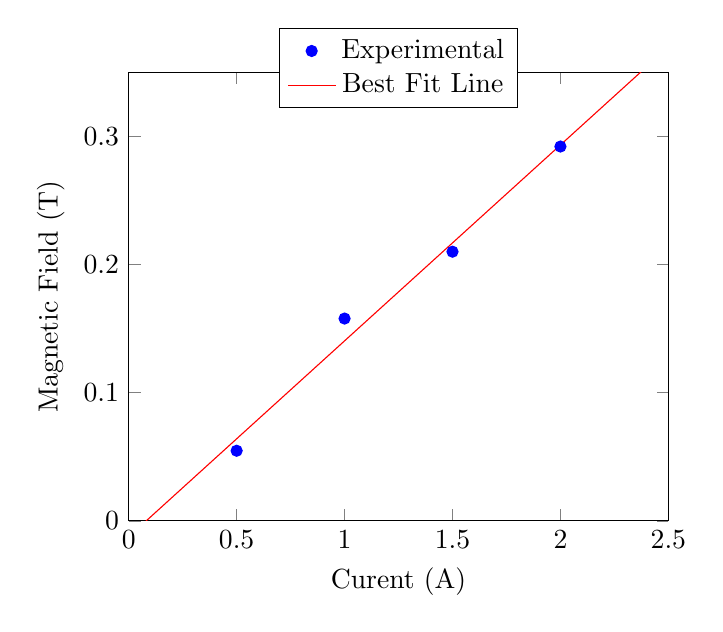
\begin{tikzpicture}
               \begin{axis}[
                  xlabel=Curent (\si{\ampere}),
                  ylabel=Magnetic Field (\si{\tesla}),
                  xmin=0,
                  xmax=2.5,
                  ymin=0,
                  ymax=.35,
                  legend pos=north west,
                  legend style={at={(0.5,1.1)},anchor=north},
                  ]
                  % Plot data
                  \addplot[only marks,mark=*,color=blue] coordinates {(0.5,0.0547) (1.0,0.1579) (1.5,0.2101) (2.0,0.2922)};

                  % Plot best fit line y=mx+b
                  \addplot[domain=0:2.5,smooth,red] {0.15294*x-0.01245};
                  \addlegendentry{Experimental}
                  \addlegendentry{Best Fit Line}
               \end{axis}
            \end{tikzpicture}
            \caption{Magnetic Field and Current Relationship in Solenoid}
            \label{fig:currentPlot}
         \end{figure}
         Magnetic field is directly proportional to the current through the solenoid.
         \item \textbf{Determine the equation of the best-fit line, including the y-intercept. Note the constants and
         their units.}

         The equation of the best-fit line is: $B(I) = 0.15294I - 0.01245$.
         \item \textbf{For each of the measurements of Part II, calculate the number of turns per meter. Enter these
         values in the data table.}
         \item \textbf{Plot a graph of magnetic field $B$ vs. the turns per meter of the solenoid ($n$).}
         \item \textbf{How is magnetic field related to the turns/meter of the solenoid?}
         \item \textbf{Determine the equation of the best-fit line to your graph. Note the constants and their units.}
         \item \textbf{From Ampere's law, it can be shown that the magnetic field $B$ inside a long solenoid
         is $B =\mu_0 n I$ where $\mu_0$ isthe permeability constant. Do your results agree with this equation? Explain.}
         \item \textbf{Assuming the equation in the previous question applies for your solenoid, calculate the value
         of $\mu_0$ using your graph of $B$ vs. $n$.}
         \item \textbf{Look up the value of $\mu_0$, the permeability constant. Compare it to your experimental value.}
         \item \textbf{Was your Slinky positioned along an east-west, north-south, or on some other axis? Will this
         have any effect on your readings?}
     \end{enumerate}
     
     \section{Extensions}
     \begin{enumerate}[1.]
      \item \textbf{Carefully measure the magnetic field at the end of the solenoid. How does it compare to the
      value at the center of the solenoid? Try to prove what the value at the end should be.}
      \item \textbf{Study the magnetic field strength inside and around a toroid, a circular-shaped solenoid.}
      \item \textbf{If you have studied calculus, refer to a calculus-based physics text to see how the equation for
      the field of a solenoid can be derived from Ampere's law.}
      \item \textbf{If you look up the permeability constant in a reference, you may find it listed in units
      of henry/meter. Show that these units are the same as tesla-meter/ampere.}
      \item \textbf{Take data on the magnetic field intensity vs. position along the length of the solenoid. Check
      the field intensity at several distances along the axis of the Slinky past the end. Note any
      patterns you see. Plot a graph of magnetic field ($B$) vs. distance from center. How does the
      value at the end of the solenoid compare to that at the center? How does the value change as
      you move away from the end of the solenoid}
      \item \textbf{Insert a steel or iron rod inside the solenoid and see what effect that has on the field intensity.
      Be careful that the rod does not short out with the coils of the Slinky. You may need to
      change the range of the Magnetic Field Sensor.}
      \item \textbf{Use the graph obtained in Part I to determine the value of $\mu_0$.}
     \end{enumerate}

\end{document}
